% Drawing 161-6/02-3 -- folder 161-6, batch 02, archive page 21 (PDF page 22).
% Transcription: plus bas dans la marge, un cercle traversé d'un faisceau de traits presque confondus, à peu près verticaux, issus d'un même point du haut du cercle, et d'un trait oblique double qui les croise ; le haut du cercle est doublé d'un second arc à droite.
% Kind: circle crossed by nearly coincident strokes. Method 2 (schematic redraw from the facsimile). Status: ok.
% Notes: A free-hand circle (closed curve through points of his outline), doubled at the upper right by a second arc. From the top of the circle, a bundle of four nearly coincident strokes going down, each drawn on its own ink: a long one that ends heavy low in the circle, a second, heavy in its upper part, ending beside it, a third ending in a small dot, and a short heavy nearly vertical stroke ending in a blot; they cross within about a unit of each other and none is exactly a diameter. Across them, an oblique double stroke from the upper right to the lower left, heavy at its lower end. At the bottom, the stroke that comes up from the next figure (its prolonged diameter) reaches the outline. The transcription's note says « deux diamètres presque confondus »: the bundle is of three or four strokes, and the oblique stroke is separate. Redrawn 2026-11-10 (issue 128). Question settled by a machine pass on the facsimile, 2026-11-12 (page): the first circle is crossed by a bundle of three or four nearly coincident strokes from the top and by a separate oblique double stroke; the drawing stands. 2026-11-13, Claude Opus 5.5, issue 147, overlay check: not compiled (no TeX in the session); the TikZ was rasterised by a local interpreter and laid over the 299 ppi scan rendered at 400 dpi. Redrawn on the ink: each stroke of the bundle and of the double stroke found by a line detector on the scan and fitted by least squares on its own ink, the outline through points moved onto its ink (its lower right part was up to three units outside the page's); every stroke lies on its ink to within about one unit. Changed: the strokes no longer pass through one computed point; they cross where they do on the page. Not checked by a reader.
% Coordinates: 1 unit = 1 mm = 1/100 of the crop width (bbox in page fractions: [0.17, 0.305, 0.35, 0.405]).
% Redrawn by Claude (claude-fable-5-2), issue #128, 2026-11-10; not checked by a human; not compiled (no TeX in the session); overlay-checked on the scan by Claude Opus 5.5, issue #147, 2026-11-13, not compiled (no TeX in the session).
% Rights: reproduces part of the work -- behind RENDER_TRANSCRIPTS, never published by itself.
\documentclass[tikz,border=3pt]{standalone}
\usepackage{amsmath,amssymb}
\usetikzlibrary{patterns,arrows.meta}
\tikzset{pencil/.style={black!45}, struck/.style={black!35}, mpt/.style={circle,draw,inner sep=1.3pt}, pt/.style={circle,fill,inner sep=0.9pt}, opt/.style={circle,draw,fill=white,inner sep=1.1pt}}
\begin{document}
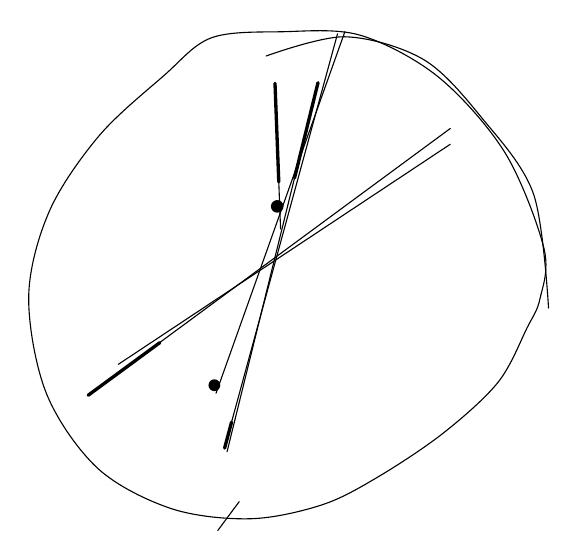
\begin{tikzpicture}[x=1mm,y=1mm,line cap=round,line join=round,font=\scriptsize]
\draw plot[smooth cycle, tension=0.55] coordinates {(41.02,-13.2) (50.01,-12.42) (59.9,-12.85) (69.86,-18.16) (78.34,-27.8) (83.28,-39.94) (82.77,-46.34) (81.13,-50.03) (77.47,-56.91) (70.52,-63.37) (62.2,-68.96) (55.1,-72.5) (46.02,-74.27) (36,-73) (26.62,-67.88) (20.09,-58.36) (17.84,-46.03) (20.48,-35.17) (26.79,-25.62) (35,-18)};
\draw plot[smooth, tension=0.55] coordinates {(48,-15.5) (58,-13.06) (68.02,-15.97) (75.46,-23.45) (81.95,-33.02) (83.86,-47.52)};
% the bundle of nearly coincident strokes from the top, each on its own ink (they cross within about a unit of each other)
\draw (57.06,-12.68) -- (43.6,-62);
\draw[very thick] (43.6,-62) -- (42.72,-65.3);
\draw (54.58,-18.89) -- (52.6,-27);
\draw[very thick] (54.58,-18.89) -- (51.6,-31);
\draw (51.6,-31) -- (43.03,-65.76);
\draw (58,-12.4) -- (41.63,-58.33);
\fill (41.42,-57.31) circle [radius=0.75];
\draw[very thick] (49.12,-18.97) -- (49.6,-31.5);
\draw (49.6,-31.5) -- (49.83,-37.47);
\fill (49.4,-34.6) circle [radius=0.8];
% the separate oblique double stroke, heavy at its lower left end
\draw (25.39,-58.59) -- (71.39,-24.7);
\draw (29.22,-54.66) -- (71.38,-26.71);
\draw[very thick] (25.39,-58.59) -- (34.5,-51.9);
% the stroke coming up from the next figure, at the bottom of the outline
\draw (44.57,-72.1) -- (41.85,-75.77);
\end{tikzpicture}
\end{document}
